%
% File Name:	pgm_overview_1.tex
% Author:	Aditya Ramesh
% Date:		06/27/2012
% Contact:	cheesear@gmail.com
%

\documentclass[11pt]{beamer}
\usepackage[noend]{algorithmic}
\usepackage{amsfonts}
\usepackage{amsmath}
\usepackage{amssymb}
\usepackage{booktabs}
\usepackage{cancel}
\usepackage{caption}
\usepackage{colortbl}
\usepackage{graphicx}
\usepackage{multirow}
\usepackage{setspace}
\usepackage{subfig}
\usepackage{tikz}
\usepackage{url}
\usepackage{xfrac}
\usetikzlibrary{calc}
\usetikzlibrary{shapes.callouts}
\usetikzlibrary{shapes.multipart}
\usetheme{Singapore}
\usecolortheme{dove}

\captionsetup[subfigure]{position=top,labelformat=empty}
\title[PGM Overview]{%
	Overview of Probabilistic Graphical Models\\
	Representation: Part I
}
\author[Aditya Ramesh]{%
	Aditya Ramesh \\
	\footnotesize\texttt{\_@adityaramesh.com}
}
\institute[University of Delaware]{%
	John Cavazos Lab\\
	University of Delaware\\
	Newark, Delaware 19716
}
\date{}
\setbeamertemplate{itemize items}{\textbullet}

\tikzset{
	darkstyle/.style={circle,draw=black,fill=white!80!black},
	lightstyle/.style={circle,draw=black,fill=white},
	tablestyle/.style={rectangle,fill=white},
	factorstyle/.style={rectangle,draw=black,fill=white!80!black}
}

\begin{document}

\begin{frame}[plain]
\titlepage
\footnotesize
This presentation is based \textbf{heavily} on the material by Daphne Koller
(\cite{pgmbook}), Nir Friedman (\cite{pgmbook}, \cite{nirslides}), and David
Sontag (\cite{pgmslides}). I have \textbf{directly copied} or otherwise
incorporated parts of their work into many of these slides, citing the sources
where appropriate. If you find this presentation useful, I highly recommend that
you take some time to read their work.
\end{frame}

\begin{frame}
\frametitle{Outline}
\tableofcontents
\end{frame}

\section{Probability Review \cite{pgmbook}}
\subsection{}

\begin{frame}{Event Spaces}
\begin{itemize}
	\item We can formalize the notion of an \emph{event} by defining a space
	of possible outcomes $\Omega$.
	\item Further, we define an \emph{event space} $S$ so that we can attach
	probabilities to specific outcomes.
	\item The event space $S$ must satisfy the following:
	\begin{itemize}
		\item $\emptyset, \Omega \in S$, where $\emptyset$ is the
		\emph{empty event} and $\Omega$ is the \emph{trivial event}.
		\item Closure under union: $\alpha, \beta \in S \rightarrow
		\alpha \cup \beta \in S$.
		\item Closure under complementation: $\alpha \in S \rightarrow
		\Omega - \alpha \in S$.
	\end{itemize}
\end{itemize}
\end{frame}

\begin{frame}{Probability Distributions}
\begin{itemize}
	\item A probability distribution over $(\Omega, S)$ is a mapping $P: S
	\rightarrow \mathbb{R}_{0}^{+}$. It must satisfy the following:
	\begin{itemize}
		\item $P(\Omega) = 1$ --- that is, the trivial event is given
		maximal probability.
		\item If $\alpha, \beta \in S$ and $\alpha \cap \beta =
		\emptyset$, then $P(\alpha \cup \beta) = P(\alpha) + P(\beta)$.
		\\ If two outcomes are mutually disjoint, the probability of
		their union is the sum of their probabilities.
		\item In this context, we view probabilities as \emph{subjective
		degrees of belief} rather than as frequencies.
	\end{itemize}
\end{itemize}
\end{frame}

\begin{frame}{Conditional Probabilities}
\begin{itemize}
	\item How are our beliefs about an outcome affected in light of new
	evidence?
	\item This notion can be formalized using the following definition,
	which relates the areas of the shaded regions in the diagram.
	\[
		P(\beta \;|\; \alpha) = \frac{P(\alpha \cap \beta)}{P(\alpha)}
	\]
	\centering
	{
		\footnotesize
		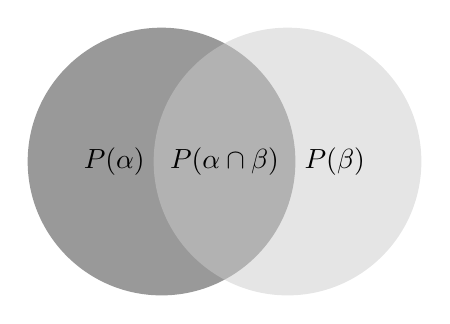
\begin{tikzpicture}
		\fill[opacity=0.5,white!20!black] (-0.8,0) circle(1.7);
		\fill[opacity=0.5,white!80!black] (0.8,0) circle(1.7);
		\node at (-1.4,0) {$P(\alpha)$};
		\node at (1.4,0) {$P(\beta)$};
		\node at (0,0) {$P(\alpha \cap \beta)$};
		\end{tikzpicture}
	}
\end{itemize}
\end{frame}

\begin{frame}{Chain Rule}
\begin{itemize}
	\item From the definition of the conditional distribution, we have
	\[
		P(\alpha \cap \beta) = P(\alpha) P(\beta \;|\; \alpha).
	\]
	\item More generally,
	\[
		P(\alpha_{1} \cap \ldots \cap \alpha_{k}) = P(\alpha_{1})
		P(\alpha_{2} \;|\; \alpha_{1}) \cdots P(\alpha_{k} \;|\;
		\alpha_{1} \cap \ldots \cap \alpha_{k - 1}),
	\]
	but the order in which we choose to pull out variables does not matter.
	\item The fact that the chain rule allows us to decompose a joint
	distribution into \emph{factors over smaller subsets of variables}
	becomes crucial later on.
\end{itemize}
\end{frame}

\begin{frame}{Bayes Rule}
\begin{itemize}
	\item Decomposing the joint distribution in the defintion of the
	conditional probability using the chain rule gives us Bayes rule:
	\[
		P(\alpha \;|\; \beta) = \frac{P(\beta \;|\; \alpha)
		P(\alpha)}{P(\beta)}.
	\]
	\item Swapping an event on the left side of the pipe symbol with an
	event on the right works similarly when we are conditioning on several
	events:
	\[
		P(\alpha \;|\; \beta \cap \gamma) = \frac{P(\beta \;|\; \alpha
		\cap \gamma) P(\alpha \;|\; \gamma)}{P(\beta \;|\; \gamma)}.
	\]
\end{itemize}
\end{frame}

\begin{frame}{Random Variables}
\begin{itemize}
	\item A random variable associates each outcome in $\Omega$ with a value
	in a discrete or continuous set, e.g. the assignment $Grade = A$ is
	shorthand for the event $\{\omega \in \Omega: f_{Grade}(\omega) = A\}$.
	\item Instead of one random variable, we can also have a random
	\emph{vector} $\boldsymbol{X}(\omega) = \{X_{1}(\omega), \ldots,
	X_{n}(\omega)\}$. Conditioning, the chain rule, and Bayes rule all
	apply \cite{pgmslides}.
	\item When dealing with categorical variables, we use $x^{i}$ to
	denote the assignment of $x$ to the $i$th state of $X$, where $i
	\in [1, |Val(X)|]$.
\end{itemize}
\end{frame}

\begin{frame}{Independence and Conditional Independence}
\begin{itemize}
	\item A distribution $P$ satisfies $(\alpha \perp \beta)$ if and only if
	$P(\alpha \cap \beta) = P(\alpha)P(\beta)$.
	\item A distribution $P$ satisfies $(\alpha \perp \beta \;|\; \gamma)$
	if and only if $P(\alpha \cap \beta \;|\; \gamma) = P(\alpha \;|\;
	\gamma)P(\beta \;|\; \gamma)$.
	\item Note the relationship between independence of variables and
	factorization of the joint distribution --- it will play a very
	prominent role later on.
\end{itemize}
\end{frame}

\section{Bayesian Networks \cite{pgmbook}}
\subsection{Introduction}

\begin{frame}{What is a Bayesian Network?}
\begin{itemize}
	\item A Bayesian Network is a directed acyclic graph (DAG) that we use
	to encode the factorization and (equivalently) the independence
	assertions of a joint distribution $P$.
	\item The nodes of the DAG are the random variables in our domain, and
	there is one CPD defined per node.
\end{itemize}
\end{frame}

\newcommand{\studentmodel}
{
	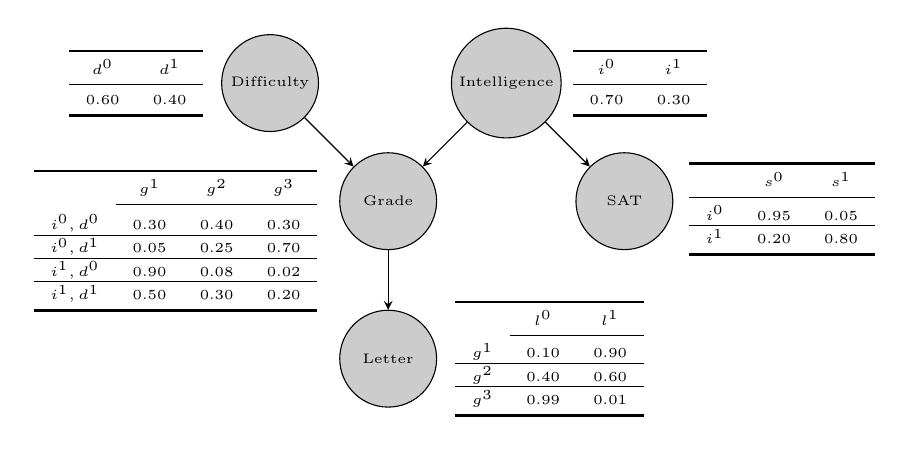
\begin{tikzpicture}
	\tiny
	\node[darkstyle,minimum size=35] (d) at (-1.5,1.5) {Difficulty};
	\node[darkstyle,minimum size=35] (i) at (1.5,1.5) {Intelligence};
	\node[darkstyle,minimum size=35] (g) at (0,0) {Grade};
	\node[darkstyle,minimum size=35] (l) at (0,-2) {Letter};
	\node[darkstyle,minimum size=35] (s) at (3,0) {SAT};
	\node[tablestyle] (dt) at (-3.2,1.5) {
		\tiny
		\begin{tabular}{cc}
		\toprule
		$d^{0}$ & $d^{1}$ \\
		\midrule
		0.60 & 0.40 \\
		\bottomrule
		\end{tabular}
	};
	\node[tablestyle] (it) at (3.2,1.5) {
		\tiny
		\begin{tabular}{cc}
		\toprule
		$i^{0}$ & $i^{1}$ \\
		\midrule
		0.70 & 0.30 \\
		\bottomrule
		\end{tabular}
	};
	\node[tablestyle] (gt) at (-2.7,-0.5) {
		\tiny
		\begin{tabular}{cccc}
		\toprule
		& $g^{1}$ & $g^{2}$ & $g^{3}$ \\
		\cmidrule{2-4}
		\noalign{\vspace{1pt}}
		$i^{0},d^{0}$ & 0.30 & 0.40 & 0.30 \\
		\hline
		\noalign{\vspace{1pt}}
		$i^{0},d^{1}$ & 0.05 & 0.25 & 0.70 \\
		\hline
		\noalign{\vspace{1pt}}
		$i^{1},d^{0}$ & 0.90 & 0.08 & 0.02 \\
		\hline
		\noalign{\vspace{1pt}}
		$i^{1},d^{1}$ & 0.50 & 0.30 & 0.20 \\
		\bottomrule
		\end{tabular}
	};
	\node[tablestyle] (lt) at (2.05,-2) {
		\tiny
		\begin{tabular}{ccc}
		\toprule
		& $l^{0}$ & $l^{1}$ \\
		\cmidrule{2-3}
		$g^{1}$ & 0.10 & 0.90 \\
		\hline
		\noalign{\vspace{1pt}}
		$g^{2}$ & 0.40 & 0.60 \\
		\hline
		\noalign{\vspace{1pt}}
		$g^{3}$ & 0.99 & 0.01 \\
		\bottomrule
		\end{tabular}
	};
	\node[tablestyle] (st) at (5,-0.1) {
		\tiny
		\begin{tabular}{ccc}
		\toprule
		& $s^{0}$ & $s^{1}$ \\
		\midrule
		$i^{0}$ & 0.95 & 0.05 \\
		\hline
		\noalign{\vspace{1pt}}
		$i^{1}$ & 0.20 & 0.80 \\
		\bottomrule
		\end{tabular}
	};
	\draw[-stealth] (d)--(g);
	\draw[-stealth] (i)--(g);
	\draw[-stealth] (i)--(s);
	\draw[-stealth] (g)--(l);
	\end{tikzpicture}
}

\begin{frame}{The Student Model}
\vspace{0pt}
\centering
\resizebox{0.8\textwidth}{!}{\studentmodel}
\begin{itemize}
	\item In the student model, $Val(D) = \{easy,hard\}, Val(I) =
	\{low,high\}, Val(G) = \{A,B,C\}, Val(S) = \{low,high\}$, and $Val(L) =
	\{weak,strong\}$.
	\item The joint distribution is $P(i,d,g,s,l) =
	P(i)P(d)P(g\;|\;i,d)P(s\;|\;i)P(l\;|\;g)$.
\end{itemize}
\end{frame}

\begin{frame}{The Student Model}
\vspace{0pt}
\centering
\resizebox{0.8\textwidth}{!}{\studentmodel}
\begin{itemize}
	\item Suppose that initially, we only have a student's recommendation
	letter (which is weak) and transcript (indicating that he received a `C'
	in the course). How does finding that he received a high SAT score
	affect our beliefs about his intelligence?
\end{itemize}
\end{frame}

\begin{frame}{The Student Model}
\vspace{0pt}
\centering
\resizebox{0.8\textwidth}{!}{\studentmodel}
\begin{itemize}
	\item What is the largest set $\boldsymbol{W}$ such that
	\begin{itemize}
		\item $(L \perp	\boldsymbol{W} \;|\; G)$?
		\item $(S \perp \boldsymbol{W} \;|\; I)$?
		\item $(G \perp \boldsymbol{W} \;|\; \pi(G))$, where $\pi(G)$
		returns the set of parents of $G$?
		\item $(D \perp \boldsymbol{W})$?
		\item $(D \perp \boldsymbol{W} \;|\; L)$?
	\end{itemize}
\end{itemize}
\end{frame}

\subsection{I-Map to Factorization}

\begin{frame}{Conclusions from the Student Model}
\begin{itemize}
	\item We view a Bayesian network as a generative model in which we
	sample the variables in topological order \cite{pgmslides}.
	\item The parents can be thought of as ``generating'' their children ---
	that is, once we know about the values of the parents, the child is
	``shielded'' from probabilistic influence by non-descendants.
	\item Consequently, we can think of a Bayesian network as representing a
	set of conditional independence assertions.
\end{itemize}
\end{frame}

\begin{frame}{I-Maps}
\begin{itemize}
	\item A Bayesian network structure $G$ encodes the following set of
	conditional independence assertions $I_{\ell}(G)$, called the
	\emph{local independencies}:
	\[
		\forall X_{i} \in Val(X): (X_{i} \perp
		\text{NonDescendants}_{X_{i}} \;|\; \pi(X_{i})).
	\]
	\item We define $I(P)$ to be the set of independence assertions of the
	form $(\boldsymbol{X} \perp \boldsymbol{Y} \;|\; \boldsymbol{Z})$ that
	hold in $P$. Obviously $I_{\ell}(G) \subseteq I(P)$.
\end{itemize}
\end{frame}

\begin{frame}{I-Maps}
\begin{itemize}
	\item Let $K$ be any graph object associated with a set of
	independencies $I(K)$. We say that $K$ is an I-map for a set of
	independencies $I$ if $I(K) \subseteq I$.
	\item That is, all the conditional independence assertions that hold in
	$I(K)$ also hold in $I$.
\end{itemize}
\end{frame}

\begin{frame}{I-Maps and Factorization}
\begin{itemize}
	\item Given that $G$ is an I-map for $P$, can we simplify the
	representation of $P$ \cite{nirslides}?
	\item Applying $I_{\ell}(G)$ to each factor in the naive decomposition
	proves that if $G$ is an I-map for $P$, then $P$ factorizes according to
	$G$. That is,
	\[
		P(X_{1}, \ldots, X_{n}) = \prod_{i=1}^{n} P(X_{i} \;|\; \pi(X_{i})).
	\]
	\item The converse is also true.
	\item The compact factorization can result in an exponential reduction
	in the number of parameters that need to be specified!
\end{itemize}
\end{frame}

\subsection{Factorization to I-Map}

\begin{frame}{I-Maps and Factorization}
\begin{itemize}
	\item Can we go the other way around and recover the graph $G$ given the
	factorization of the distribution $P$?
	\item We will first take a detour and explore more deeply how
	probabilistic influence flows across a graph.
\end{itemize}
\end{frame}

\captionsetup[subfigure]{position=bottom,labelformat=parens}

\newcommand{\trailseries}
{
	\subfloat[][]{
		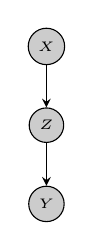
\begin{tikzpicture}[every node/.style=
		{
			circle,
			draw=black,
			fill=white!80!black
		}]
		\tiny
		\node (x) at (0,1.0) {$X$};
		\node (z) at (0,0) {$Z$};
		\node (y) at (0,-1.0) {$Y$};
		\draw[-stealth] (x)--(z);
		\draw[-stealth] (z)--(y);
		\end{tikzpicture}
	}%
	\hspace{0.4cm}
	\subfloat[][]{
		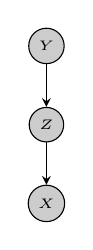
\begin{tikzpicture}[every node/.style=
		{
			circle,
			draw=black,
			fill=white!80!black
		}]
		\tiny
		\node (y) at (0,1.0) {$Y$};
		\node (z) at (0,0) {$Z$};
		\node (x) at (0,-1.0) {$X$};
		\draw[-stealth] (y)--(z);
		\draw[-stealth] (z)--(x);
		\end{tikzpicture}
	}%
	\hspace{0.4cm}
	\subfloat[][]{
		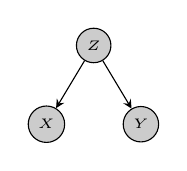
\begin{tikzpicture}[every node/.style=
		{
			circle,
			draw=black,
			fill=white!80!black
		}]
		\tiny
		\node (x) at (-0.6,0) {$X$};
		\node (z) at (0,1) {$Z$};
		\node (y) at (0.6,0) {$Y$};
		\draw[-stealth] (z)--(x);
		\draw[-stealth] (z)--(y);
		\end{tikzpicture}
	}%
	\subfloat[][]{
		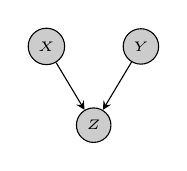
\begin{tikzpicture}[every node/.style=
		{
			circle,
			draw=black,
			fill=white!80!black
		}]
		\tiny
		\node (x) at (-0.6,1) {$X$};
		\node (z) at (0,0) {$Z$};
		\node (y) at (0.6,1) {$Y$};
		\draw[-stealth] (x)--(z);
		\draw[-stealth] (y)--(z);
		\end{tikzpicture}
	}
}

\begin{frame}{Path Blockage \cite{nirslides}}
\vspace{0pt}
\setlength{\topsep}{0pt}
\setlength{\partopsep}{0pt}
\begin{figure}[!t]
\centering
\trailseries
\caption*{\scriptsize The four possible edge trail combinations from $X$ to $Y$
via $Z$: (a) An indirect causal effect; (b) An indirect evidential effect; (c) A
common cause; (d) A common effect.}
\end{figure}
\begin{itemize}
	\item Edge trails (a)--(c) are active if and only if $Z$ is not
	observed.
	\item Edge trail (d) is active if and only if either $Z$ or one of $Z$'s
	descendants is observed. Intuitively, this can be understood as a
	consequence of intercausual reasoning.
\end{itemize}
\end{frame}

\begin{frame}{Path Blockage}
\begin{itemize}
	\item Now we can extend our finding about three-node edge-trails to
	trails of arbitrary length.
	\item The trail $X_{1} \leftrightharpoons \cdots \leftrightharpoons
	X_{n}$ is active given a subset of observed variables $\boldsymbol{Z}$
	if
	\begin{itemize}
		\item Whenever we have a v-structure $X_{i-1} \rightarrow X_{i}
		\leftarrow X_{i+1}$, then $X_{i}$ or one of its descendants are
		in $\boldsymbol{Z}$.
		\item No other node along the trail is in $\boldsymbol{Z}$.
	\end{itemize}
\end{itemize}
\end{frame}

\begin{frame}{D-Separation}
\begin{itemize}
	\item We say that $\boldsymbol{X}$ and $\boldsymbol{Y}$ are d-separated
	(``directed-separated'') given $\boldsymbol{Z}$, denoted
	$\text{d-sep}_{G}(\boldsymbol{X};\boldsymbol{Y}\;|\;\boldsymbol{Z})$, if
	there is no active trail between any node $X \in \boldsymbol{X}$ and $Y
	\in \boldsymbol{Y}$ given $\boldsymbol{Z}$.
	\item We use $I(G)$ to denote the set of independencies (aka
	\emph{global Markov independencies}) that correspond to d-separation:
	\[
		I(G) = \{(\boldsymbol{X} \perp \boldsymbol{Y} \;|\;
		\boldsymbol{Z}) : \text{d-sep}_{G}(\boldsymbol{X};
		\boldsymbol{Y} \;|\; \boldsymbol{Z})\}.
	\]
\end{itemize}
\end{frame}

\begin{frame}{D-Separation \cite{pgmslides}}
\resizebox{\textwidth}{!}
{
	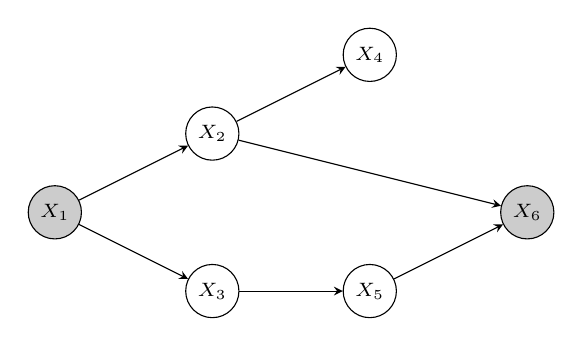
\begin{tikzpicture}
	\scriptsize
	\node[darkstyle] (x1) at (-3,0) {$X_{1}$};
	\node[lightstyle] (x2) at (-1,1) {$X_{2}$};
	\node[lightstyle] (x3) at (-1,-1) {$X_{3}$};
	\node[lightstyle] (x4) at (1,2) {$X_{4}$};
	\node[lightstyle] (x5) at (1,-1) {$X_{5}$};
	\node[darkstyle] (x6) at (3,0) {$X_{6}$};
	\draw[-stealth] (x1)--(x2);
	\draw[-stealth] (x1)--(x3);
	\draw[-stealth] (x2)--(x4);
	\draw[-stealth] (x2)--(x6);
	\draw[-stealth] (x3)--(x5);
	\draw[-stealth] (x5)--(x6);
	\end{tikzpicture}
}
\end{frame}

\begin{frame}{Independence and D-Separation}
\begin{itemize}
	\item We now return to make the connection between the factorization of
	$P$ and the construction of $G$.
	\item For any distribution $G$ that factorizes over $G$, we have that
	we have that if $X$ and $Y$ are not d-separated given $\boldsymbol{Z}$
	in $G$, then $X$ and $Y$ are dependent in all distributions $P$ that
	factorize over $G$.
	\item Otherwise, $G$ would contain some independence assertion that is
	not reflected in $P$, a contradiction.
\end{itemize}
\end{frame}

\begin{frame}{Independence and D-Separation}
\begin{itemize}
	\item For almost all distributions $P$ that factorize over $G$, that is,
	for all distributions except for a set of measure zero in the space of
	CPD parameterizations, we have that $I(P) = I(G)$.
	\item D-separation reduces statistical independencies in graphs (hard)
	to connectivity in graphs (easy) \cite{pgmslides}.
\end{itemize}
\end{frame}

%\begin{frame}{Independence and D-Separation}
%\begin{itemize}
%	\item Answering the question of how we can recover $G$ given the
%	factorization of $P$ requires learning about minimal I-maps and their
%	construction.
%	\item A graph $G$ can have several minimal I-maps, so we require the
%	concept of a P-map in order to guarantee uniqueness and form an
%	equivalence relation among DAGs.
%	\item Refer to Chapter 3 of \cite{pgmbook} and \cite{arslides} for more
%	information.
%\end{itemize}
%\end{frame}

\newcommand{\completedag}
{
	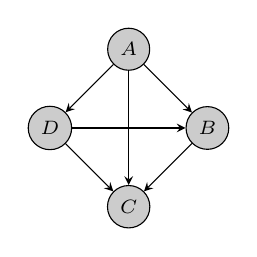
\begin{tikzpicture}
	\scriptsize
	\node[darkstyle] (a) at (0,1) {$A$};
	\node[darkstyle] (b) at (1,0) {$B$};
	\node[darkstyle] (c) at (0,-1) {$C$};
	\node[darkstyle] (d) at (-1,0) {$D$};
	\draw[-stealth] (a)--(b);
	\draw[-stealth] (a)--(d);
	\draw[-stealth] (b)--(c);
	\draw[-stealth] (d)--(c);
	\draw[-stealth] (a)--(c);
	\draw[-stealth] (d)--(b);
	\end{tikzpicture}
}

\begin{frame}{Minimal I-Maps \cite{nirslides}}
\setlength{\topsep}{0pt}
\setlength{\partopsep}{0pt}
\vspace{0pt}
\centering
\resizebox{!}{0.35\textheight}{\completedag}
\begin{itemize}
	\item By itself, the concept of an I-map is not sufficient for us to get
	very far.
	\item The graph depicted above (a \emph{complete} DAG) is an I-map for
	\emph{any} distribution $P$.
\end{itemize}
\end{frame}

\begin{frame}{Minimal I-Maps \cite{nirslides}}
\begin{itemize}
	\item A graph $K$ is a minimal I-map for a set of independence
	assertions $I$ if $K$ is an I-map for $I$, and the removal of even a
	single edge from $K$ renders it not an I-map.
	\item Taking $I = I(P)$ or $I = I(K')$, we can talk about $K$ as being a
	minimal I-map for a distribution or another graph.
\end{itemize}
\end{frame}

\begin{frame}{Algorithm for Constructing a Minimal I-Map}
\setlength{\topsep}{0pt}
\setlength{\partopsep}{0pt}
\vspace{0pt}
\begin{algorithmic}
\REQUIRE An ordering $X_{1}, \ldots, X_{n}$ of random variables in $\mathcal{X}$
\REQUIRE A set of independencies $I$
\pause
\STATE Set $G$ to an empty graph over $\mathcal{X}$
\pause
\FOR{$i = 1, \ldots, n$}
	\STATE{\textcolor{gray}{$\boldsymbol{U}$ is the current candidate for
	parents of $X_{i}$}}
	\STATE $\boldsymbol{U} \leftarrow \{X_{1}, \ldots, X_{i-1}\}$
	\pause
	\STATE{\textcolor{gray}{Find the minimal set $\boldsymbol{U}$ satisfying
	$(X_{i} \perp \{X_{1}, \ldots, X_{i-1}\} - \boldsymbol{U} \;|\;
	\boldsymbol{U})$}}
	\FOR{$\boldsymbol{U'} \subseteq \{X_{1}, \ldots, X_{i-1}\}$}
		\IF{$\boldsymbol{U'} \subset \boldsymbol{U}$ and $(X_{i} \perp
		\{X_{1}, \ldots, X_{i-1}\} - \boldsymbol{U'} \;|\;
		\boldsymbol{U'}) \in I$}
			\STATE{$\boldsymbol{U} \leftarrow \boldsymbol{U'}$}
		\ENDIF
	\ENDFOR
	\pause
	\STATE{\textcolor{gray}{Now set $\boldsymbol{U}$ to be the parents of
	$X_{i}$}}
	\FOR{$X_{i} \in \boldsymbol{U}$}
		\STATE{Add $X_{j} \text{---} X_{i}$ to $G$}
	\ENDFOR
	\pause
	\RETURN{$G$}
\ENDFOR
\end{algorithmic}
\end{frame}

\begin{frame}{Constructing a Minimal I-Map}
\vspace{0pt}
\centering
\resizebox{0.8\textwidth}{!}{\studentmodel}
\begin{itemize}
	\item We now apply the algorithm to the variables in the student model,
	listed in topological order: $D,I,S,G,L$.
\end{itemize}
\end{frame}

\begin{frame}{Constructing a Minimal I-Map}
\centering
\begin{figure}
\centering
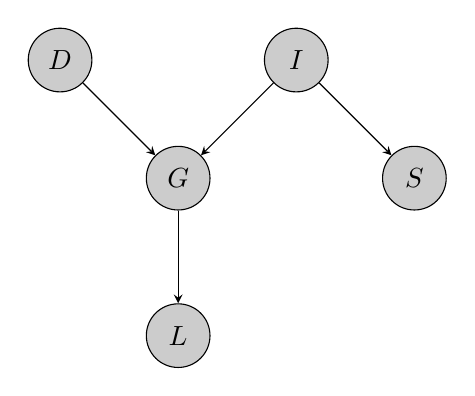
\begin{tikzpicture}
\normalsize
\node[darkstyle,minimum size=23] (d) at (-1.5,1.5) {$D$};
\pause
\node[darkstyle,minimum size=23] (i) at (1.5,1.5) {$I$};
\pause
\node[darkstyle,minimum size=23] (s) at (3,0) {$S$};
\pause
\draw[-stealth] (i)--(s);
\pause
\node[darkstyle,minimum size=23] (g) at (0,0) {$G$};
\pause
\draw[-stealth] (d)--(g);
\pause
\draw[-stealth] (i)--(g);
\pause
\node[darkstyle,minimum size=23] (l) at (0,-2) {$L$};
\pause
\draw[-stealth] (g)--(l);
\end{tikzpicture}
\end{figure}
\end{frame}

\begin{frame}{Constructing a Minimal I-Map}
\begin{itemize}
	\item If we run the algorithm with an ordering that is topological for
	$G$, then the algorithm returns $G$.
	\item This is because the set of parents that are considered for each
	$X_{i}$ is precisely $\pi(X_{i})$.
	\item Now, we consider a less natural ordering: $L,D,S,I,G$.
\end{itemize}
\end{frame}

\begin{frame}{Constructing a Minimal I-Map}
\centering
\begin{figure}
\centering
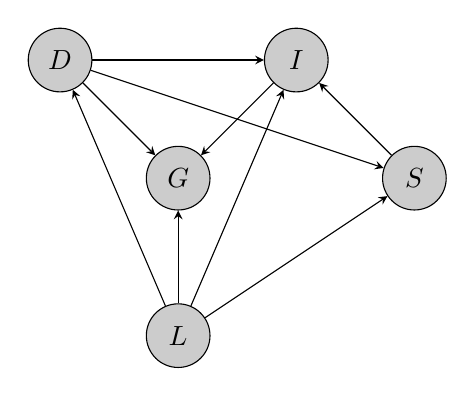
\begin{tikzpicture}
\normalsize
\node[darkstyle,minimum size=23] (l) at (0,-2) {$L$};
\pause
\node[darkstyle,minimum size=23] (d) at (-1.5,1.5) {$D$};
\pause
\draw[-stealth] (l)--(d);
\pause
\node[darkstyle,minimum size=23] (s) at (3,0) {$S$};
\pause
\draw[-stealth] (l)--(s);
\pause
\draw[-stealth] (d)--(s);
\pause
\node[darkstyle,minimum size=23] (i) at (1.5,1.5) {$I$};
\pause
\draw[-stealth] (l)--(i);
\pause
\draw[-stealth] (d)--(i);
\pause
\draw[-stealth] (s)--(i);
\pause
\node[darkstyle,minimum size=23] (g) at (0,0) {$G$};
\pause
\draw[-stealth] (l)--(g);
\pause
\draw[-stealth] (d)--(g);
\pause
\draw[-stealth] (i)--(g);
\end{tikzpicture}
\end{figure}
\end{frame}

\captionsetup[subfigure]{position=bottom,labelformat=empty}

\begin{frame}{Construction of Minimal I-Maps}
\centering
\begin{figure}
\resizebox{0.6\textwidth}{!}{
\subfloat[][(a)]
{%
	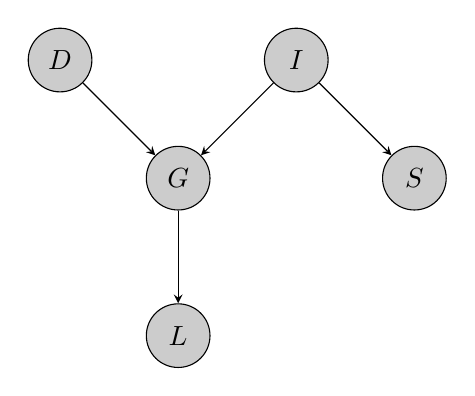
\begin{tikzpicture}
	\normalsize
	\node[darkstyle,minimum size=23] (d) at (-1.5,1.5) {$D$};
	\node[darkstyle,minimum size=23] (i) at (1.5,1.5) {$I$};
	\node[darkstyle,minimum size=23] (s) at (3,0) {$S$};
	\draw[-stealth] (i)--(s);
	\node[darkstyle,minimum size=23] (g) at (0,0) {$G$};
	\draw[-stealth] (d)--(g);
	\draw[-stealth] (i)--(g);
	\node[darkstyle,minimum size=23] (l) at (0,-2) {$L$};
	\draw[-stealth] (g)--(l);
	\end{tikzpicture}
}%
\subfloat[][(b)]
{%
	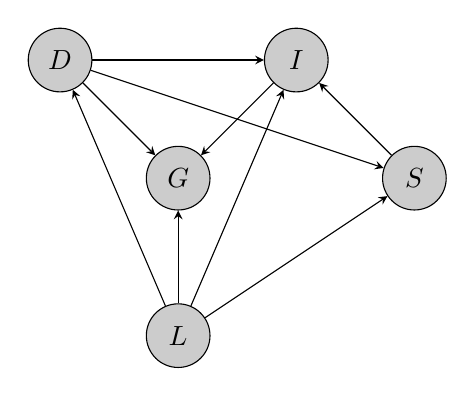
\begin{tikzpicture}
	\normalsize
	\node[darkstyle,minimum size=23] (l) at (0,-2) {$L$};
	\node[darkstyle,minimum size=23] (d) at (-1.5,1.5) {$D$};
	\draw[-stealth] (l)--(d);
	\node[darkstyle,minimum size=23] (s) at (3,0) {$S$};
	\draw[-stealth] (l)--(s);
	\draw[-stealth] (d)--(s);
	\node[darkstyle,minimum size=23] (i) at (1.5,1.5) {$I$};
	\draw[-stealth] (l)--(i);
	\draw[-stealth] (d)--(i);
	\draw[-stealth] (s)--(i);
	\node[darkstyle,minimum size=23] (g) at (0,0) {$G$};
	\draw[-stealth] (l)--(g);
	\draw[-stealth] (d)--(g);
	\draw[-stealth] (i)--(g);
	\end{tikzpicture}
}
}
\end{figure}
\begin{itemize}
	\item Both graphs (a) and (b) are valid I-maps for $G$, but have
	completely different edge configurations.
	\item Ironically, we cannot ``read off'' the independence assertions
	from a minimal I-map. Even minimal I-maps fail to capture some or all of
	the independencies that hold in the distribution.
\end{itemize}
\end{frame}

\begin{frame}{Constructing Minimal I-Maps}
\begin{itemize}
	\item A more restrictive definition called the perfect map (P-map)
	captures the independencies in a given distribution $P$.
	\item We say that a graph $K$ is a P-map for $P$ if $I(K) = I(P)$.
	\item Through an involved process, it is possible to construct a PDAG
	(partially directed acyclic graph) from a distribution $P$ that encodes
	all P-maps in the I-equivalence class of $P$.
	\item Unfortunately, not all distributions have P-maps.
\end{itemize}
\end{frame}

\subsection{Applications}

\newcommand{\naivebayes}
{
	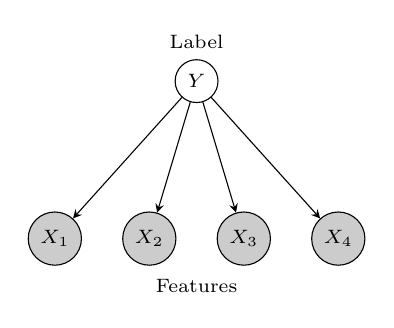
\begin{tikzpicture}
	\scriptsize
	\node[lightstyle] (y) at (0,2.0) {$Y$};
	\node[darkstyle] (x1) at (-1.8,0) {$X_{1}$};
	\node[darkstyle] (x2) at (-0.6,0) {$X_{2}$};
	\node[darkstyle] (x3) at (0.6,0) {$X_{3}$};
	\node[darkstyle] (x4) at (1.8,0) {$X_{4}$};
	\node at (0,2.5) {Label};
	\node at (0,-0.6) {Features};
	\draw[-stealth] (y)--(x1);
	\draw[-stealth] (y)--(x2);
	\draw[-stealth] (y)--(x3);
	\draw[-stealth] (y)--(x4);
	\end{tikzpicture}
}

\begin{frame}{Email Classification \cite{pgmslides}}
\setlength{\topsep}{0pt}
\setlength{\partopsep}{0pt}
\vspace{0pt}
\centering
\resizebox{!}{0.35\textheight}{\naivebayes}
\begin{itemize}
	\item We now shift our focus to a few applications of Bayesian networks.
	\item To generate an email, recall that we can sample the variables in
	the Bayesian network in topological order.
	\begin{itemize}
		\item First, we sample $y \sim P(Y)$ to decide whether or not
		the email is spam.
		\item Then, $\forall i \in [1,n]$ sample $x_{i} \sim P(X_{i}
		\;|\; Y=y)$.
	\end{itemize}
\end{itemize}
\end{frame}

\begin{frame}{Email Classification \cite{pgmslides}}
\setlength{\topsep}{0pt}
\setlength{\partopsep}{0pt}
\vspace{0pt}
\centering
\resizebox{!}{0.35\textheight}{\naivebayes}
\begin{itemize}
	\item To determine whether an email is spam given the features
	$\boldsymbol{X}_{i}$, we need to compute
	\begin{align*}
		P(Y \;|\; \boldsymbol{X}_{i}) &=
		\frac{P(Y, \boldsymbol{X}_{i})}{P(\boldsymbol{X}_{i})} \\
		&= \frac{P(Y) \prod_{i=1}^{n} P(Y \;|\; X_{i})}
		{\sum_{y \in Y} P(Y, \boldsymbol{X}_{i})} \\
		&= \frac{P(Y) \prod_{i=1}^{n} P(Y \;|\; X_{i})}
		{\sum_{y \in Y} P(Y) \prod_{i=1}^{n} P(Y \;|\; X_{i})}.
	\end{align*}
\end{itemize}
\end{frame}

\begin{frame}{Email Classification}
\begin{itemize}
	\item We can view every email in our corpus as a bag of words and let
	the features $\boldsymbol{X}_{i}$ be functions of their counts (e.g.
	``Nigeria'', ``bank'').
	\item The local probability models (in our case $P(Y)$ and $P(X_{i}
	\;|\; Y) \;\forall X_{i}$) are now easily computed, and we have designed a
	primitive email spam-detection system.
	\item What is the name of this classifier?
\end{itemize}
\end{frame}

\newcommand{\medicaldiagnosis}
{
	\centering
	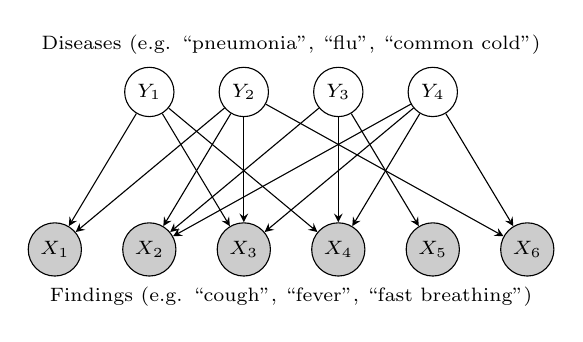
\begin{tikzpicture}
	\scriptsize
	\node[lightstyle] (y1) at (-1.8,2) {$Y_{1}$};
	\node[lightstyle] (y2) at (-0.6,2) {$Y_{2}$};
	\node[lightstyle] (y3) at (0.6,2) {$Y_{3}$};
	\node[lightstyle] (y4) at (1.8,2) {$Y_{4}$};
	\node[darkstyle] (x1) at (-3.0,0) {$X_{1}$};
	\node[darkstyle] (x2) at (-1.8,0) {$X_{2}$};
	\node[darkstyle] (x3) at (-0.6,0) {$X_{3}$};
	\node[darkstyle] (x4) at (0.6,0) {$X_{4}$};
	\node[darkstyle] (x5) at (1.8,0) {$X_{5}$};
	\node[darkstyle] (x6) at (3.0,0) {$X_{6}$};
	\node at (0,2.6) {Diseases (e.g. ``pneumonia'', ``flu'', ``common
	cold'')};
	\node at (0,-0.6) {Findings (e.g. ``cough'', ``fever'', ``fast
	breathing'')};
	\draw[-stealth] (y1)--(x1);
	\draw[-stealth] (y1)--(x3);
	\draw[-stealth] (y1)--(x4);
	\draw[-stealth] (y2)--(x1);
	\draw[-stealth] (y2)--(x2);
	\draw[-stealth] (y2)--(x3);
	\draw[-stealth] (y2)--(x6);
	\draw[-stealth] (y3)--(x2);
	\draw[-stealth] (y3)--(x4);
	\draw[-stealth] (y3)--(x5);
	\draw[-stealth] (y4)--(x2);
	\draw[-stealth] (y4)--(x3);
	\draw[-stealth] (y4)--(x4);
	\draw[-stealth] (y4)--(x6);
	\end{tikzpicture}
}

\begin{frame}{Naive Bayes \cite{pgmslides}}
\setlength{\topsep}{0pt}
\setlength{\partopsep}{0pt}
\vspace{0pt}
\centering
\resizebox{\textwidth}{!}{\medicaldiagnosis}
\end{frame}

\section{Markov Networks \cite{pgmbook}}
\subsection{Introduction}

\captionsetup[subfigure]{position=bottom,labelformat=empty}

\newcommand{\misconception}
{
	\begin{centering}
	\subfloat[][(a)]{%
		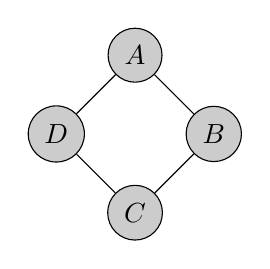
\begin{tikzpicture}
		\node[darkstyle] (a) at (0,1) {$A$};
		\node[darkstyle] (b) at (1,0) {$B$};
		\node[darkstyle] (c) at (0,-1) {$C$};
		\node[darkstyle] (d) at (-1,0) {$D$};
		\draw (a)--(b);
		\draw (b)--(c);
		\draw (c)--(d);
		\draw (d)--(a);
		\end{tikzpicture}
	}
	\hspace{0.3cm}
	\subfloat[][(b)]{%
		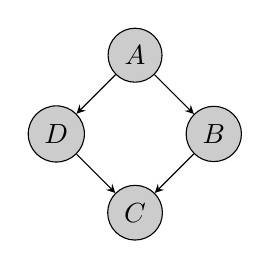
\begin{tikzpicture}
		\node[darkstyle] (a) at (0,1) {$A$};
		\node[darkstyle] (b) at (1,0) {$B$};
		\node[darkstyle] (c) at (0,-1) {$C$};
		\node[darkstyle] (d) at (-1,0) {$D$};
		\draw[-stealth] (a)--(b);
		\draw[-stealth] (a)--(d);
		\draw[-stealth] (b)--(c);
		\draw[-stealth] (d)--(c);
		\end{tikzpicture}
	}
	\hspace{0.3cm}
	\subfloat[][(c)]{
		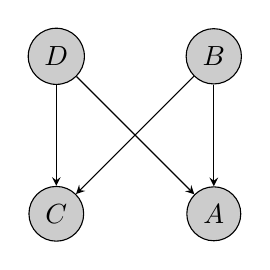
\begin{tikzpicture}
		\node[darkstyle] (d) at (-1,1) {$D$};
		\node[darkstyle] (b) at (1,1) {$B$};
		\node[darkstyle] (a) at (1,-1) {$A$};
		\node[darkstyle] (c) at (-1,-1) {$C$};
		\draw[-stealth] (d)--(c);
		\draw[-stealth] (d)--(a);
		\draw[-stealth] (b)--(c);
		\draw[-stealth] (b)--(a);
		\end{tikzpicture}
	}
	\end{centering}
}

\begin{frame}{Motivation}
\setlength{\topsep}{0pt}
\setlength{\partopsep}{0pt}
\vspace{0pt}
\centering
\begin{figure}[!t]
\scriptsize
\resizebox{0.8\textwidth}{!}{\misconception}
\caption*{\scriptsize A professor misspeaks in class, causing four students to
have a misconception. This model predicts whether or not each of them continues
to carry the misconception after the students meet in pairs (Alice and Bob, Bob
and Charles, Charles and Debbie, and Debbie and Alice).}
\end{figure}
\begin{itemize}
	\item We want to encode $(A \perp C \;|\; D,B)$ and $(B \perp D \;|\;
	A,C)$. Why do (b) and (c) fail to capture these independencies?
	\item The fact that the a CPD involving a variable in a Bayesian network
	can only be over itself and its parents poses limitations.
\end{itemize}
\end{frame}

\begin{frame}{What is a Markov Network?}
\begin{itemize}
	\item Similarly to Bayesian networks, a Markov network, or Markov random
	field (MRF) is an undirected graphical model with one node per variable.
	\item Unlike Bayesian networks, the non-negative potential functions (or
	\emph{factors}) are associated with cliques of variables.
	\[
		P(X_{1}, \ldots, X_{n}) = \frac{1}{Z} \tilde{P}(X_{1}, \ldots,
		X_{n}),
	\]
	where the normalizing constant (or \emph{partition function}) $Z$ is
	defined as
	\[
		Z = \sum_{X_{1}, \ldots, X_{n}} \tilde{P}(X_{1}, \ldots, X_{n}).
	\]
	\item A distribution of this kind is called a \emph{Gibbs distribution}.
\end{itemize}
\end{frame}

\begin{frame}{What is a Markov Network?}
\begin{itemize}
	\item Unlike Bayesian networks, the factors do not have to be
	normalized, so $\tilde{P}$ does not have to be normalized.
	\item We define the the \emph{factor product} over some
	$\phi_{1}(\boldsymbol{X}, \boldsymbol{Y})$ and $\phi_{2}(\boldsymbol{Y},
	\boldsymbol{Z})$, $\phi_{1} \times \phi_{2}$, by
	\[
		\psi(\boldsymbol{X}, \boldsymbol{Y}, \boldsymbol{Z}) =
		\phi_{1}(\boldsymbol{X}, \boldsymbol{Y}) \cdot
		\phi_{2}(\boldsymbol{Y}, \boldsymbol{Z}).
	\]
	\item Now we can define $\tilde{P}$ given a set of factors
	$\boldsymbol{\Phi} = \{\phi_{1}(\boldsymbol{D}_{1}), \ldots,
	\phi_{m}(\boldsymbol{D}_{m})\}$:
	\[
		\tilde{P}(X_{1}, \ldots, X_{n}) = \phi_{1}(\boldsymbol{D}_{1})
		\times \cdots \times \phi_{m}(\boldsymbol{D}_{m}).
	\]
\end{itemize}
\end{frame}

\newcommand{\misconceptionmrf}
{
	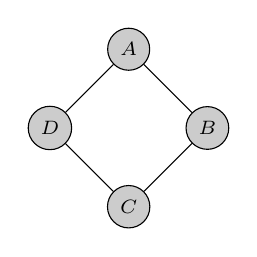
\begin{tikzpicture}
	\scriptsize
	\node[darkstyle] (a) at (0,1) {$A$};
	\node[darkstyle] (b) at (1,0) {$B$};
	\node[darkstyle] (c) at (0,-1) {$C$};
	\node[darkstyle] (d) at (-1,0) {$D$};
	\draw (a)--(b);
	\draw (b)--(c);
	\draw (c)--(d);
	\draw (d)--(a);
	\end{tikzpicture}
}

\begin{frame}{The Misconception Model \cite{pgmslides}}
\setlength{\topsep}{0pt}
\setlength{\partopsep}{0pt}
\vspace{0pt}
\centering
\begin{figure}[!t]
\resizebox{0.3\textwidth}{!}{\misconceptionmrf}
\end{figure}
\begin{itemize}
	\item We introduce single-node potentials $\phi_{A}, \phi_{B}, \phi_{C},
	\phi_{D}$ to represent probabilities that individuals correctly work out
	the misconceptions themselves.
	\item We introduce pairwise potentials $\phi_{AB}, \phi_{BC}, \phi_{CD},
	\phi_{DA}$ to model whether partners agree after their meeting.
\end{itemize}
\end{frame}

\begin{frame}{The Misconception Model \cite{pgmslides}}
\begin{itemize}
	\item The joint distribution is
	\begin{align*}
		P(A,B,C,D) &= \frac{1}{Z}\phi(a)\phi(b)\phi(c)\phi(d) \\
		&\phi(a,b)\phi(b,c)\phi(c,d)\phi(d,a).
	\end{align*}
	\item Entries in the potentials need not be normalized; we can only
	judge relative importance by normalizing (scaling by $Z$) before
	comparison.
\end{itemize}
\end{frame}

\newcommand{\factorproduct}
{
	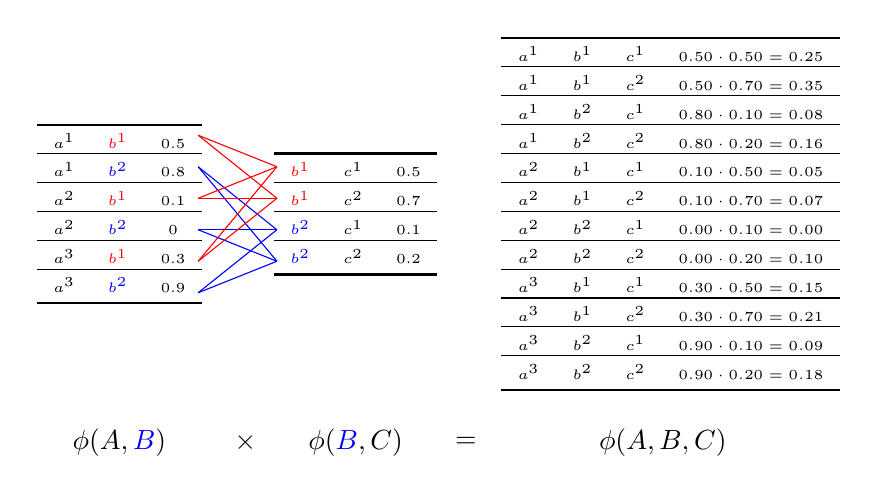
\begin{tikzpicture}
	\node[tablestyle] (a) at (-3,0) {
		\tiny
		\begin{tabular}{ccc}
		\toprule
		$a^{1}$ & \color{red}$b^{1}$ & 0.5 \\
		\hline
		\noalign{\smallskip}
		$a^{1}$ & \color{blue}$b^{2}$ & 0.8 \\
		\hline
		\noalign{\smallskip}
		$a^{2}$ & \color{red}$b^{1}$ & 0.1 \\
		\hline
		\noalign{\smallskip}
		$a^{2}$ & \color{blue}$b^{2}$ & 0 \\
		\hline
		\noalign{\smallskip}
		$a^{3}$ & \color{red}$b^{1}$ & 0.3 \\
		\hline
		\noalign{\smallskip}
		$a^{3}$ & \color{blue}$b^{2}$ & 0.9 \\
		\bottomrule
		\end{tabular}
	};
	\node[tablestyle] (b) at (0,0) {
		\tiny
		\begin{tabular}{ccc}
		\toprule
		\color{red}$b^{1}$ & $c^{1}$ & 0.5 \\
		\hline
		\noalign{\smallskip}
		\color{red}$b^{1}$ & $c^{2}$ & 0.7 \\
		\hline
		\noalign{\smallskip}
		\color{blue}$b^{2}$ & $c^{1}$ & 0.1 \\
		\hline
		\noalign{\smallskip}
		\color{blue}$b^{2}$ & $c^{2}$ & 0.2 \\
		\bottomrule
		\end{tabular}
	};
	\node[tablestyle] (c) at (4,0) {
		\tiny
		\begin{tabular}{cccc}
		\toprule
		$a^{1}$ & $b^{1}$ & $c^{1}$ & $0.50 \cdot 0.50 = 0.25$ \\
		\hline
		\noalign{\smallskip}
		$a^{1}$ & $b^{1}$ & $c^{2}$ & $0.50 \cdot 0.70 = 0.35$ \\
		\hline
		\noalign{\smallskip}
		$a^{1}$ & $b^{2}$ & $c^{1}$ & $0.80 \cdot 0.10 = 0.08$ \\
		\hline
		\noalign{\smallskip}
		$a^{1}$ & $b^{2}$ & $c^{2}$ & $0.80 \cdot 0.20 = 0.16$ \\
		\hline
		\noalign{\smallskip}
		$a^{2}$ & $b^{1}$ & $c^{1}$ & $0.10 \cdot 0.50 = 0.05$ \\
		\hline
		\noalign{\smallskip}
		$a^{2}$ & $b^{1}$ & $c^{2}$ & $0.10 \cdot 0.70 = 0.07$ \\
		\hline
		\noalign{\smallskip}
		$a^{2}$ & $b^{2}$ & $c^{1}$ & $0.00 \cdot 0.10 = 0.00$ \\
		\hline
		\noalign{\smallskip}
		$a^{2}$ & $b^{2}$ & $c^{2}$ & $0.00 \cdot 0.20 = 0.10$ \\
		\hline
		\noalign{\smallskip}
		$a^{3}$ & $b^{1}$ & $c^{1}$ & $0.30 \cdot 0.50 = 0.15$ \\
		\hline
		\noalign{\smallskip}
		$a^{3}$ & $b^{1}$ & $c^{2}$ & $0.30 \cdot 0.70 = 0.21$ \\
		\hline
		\noalign{\smallskip}
		$a^{3}$ & $b^{2}$ & $c^{1}$ & $0.90 \cdot 0.10 = 0.09$ \\
		\hline
		\noalign{\smallskip}
		$a^{3}$ & $b^{2}$ & $c^{2}$ & $0.90 \cdot 0.20 = 0.18$ \\
		\bottomrule
		\end{tabular}
	};

	\coordinate (a1) at (-2,1.0) {};
	\coordinate (a2) at (-2,0.6) {};
	\coordinate (a3) at (-2,0.2) {};
	\coordinate (a4) at (-2,-0.2) {};
	\coordinate (a5) at (-2,-0.6) {};
	\coordinate (a6) at (-2,-1.0) {};
	\coordinate (b1) at (-1.0,0.6) {};
	\coordinate (b2) at (-1.0,0.2) {};
	\coordinate (b3) at (-1.0,-0.2) {};
	\coordinate (b4) at (-1.0,-0.6) {};
	\draw[red] (a1)--(b1);
	\draw[red] (a1)--(b2);
	\draw[blue] (a2)--(b3);
	\draw[blue] (a2)--(b4);
	\draw[red] (a3)--(b1);
	\draw[red] (a3)--(b2);
	\draw[blue] (a4)--(b3);
	\draw[blue] (a4)--(b4);
	\draw[red] (a5)--(b1);
	\draw[red] (a5)--(b2);
	\draw[blue] (a6)--(b3);
	\draw[blue] (a6)--(b4);

	\node at (-3.0,-2.9) {$\phi(A,\textcolor{blue}{B})$};
	\node at (-1.4,-2.9) {$\times$};
	\node at (-0.0,-2.9) {$\phi(\textcolor{blue}{B},C)$};
	\node at (1.4,-2.9) {$=$};
	\node at (3.9,-2.9) {$\phi(A,B,C)$};
	\end{tikzpicture}
}

\begin{frame}{Factor Product}
\setlength{\topsep}{0pt}
\setlength{\partopsep}{0pt}
\vspace{0pt}
\centering
\begin{figure}[!t]
\factorproduct
\end{figure}
\end{frame}

\subsection{Independence}

\begin{frame}{Independence \cite{pgmslides}}
\begin{itemize}
	\item Consider a Markov network $A\text{---}B\text{---}C$ with the joint
	distribution
	\[
		P(a,b,c) = \frac{1}{Z}\phi_{AB}(a,b)\phi_{BC}(b,c).
	\]
	\item First, we show that $P(a \;|\; b)$ can be computed using only
	$\phi_{AB}(a,b)$:
	\begin{align*}
		P(a \;|\; b) &= \frac{P(a,b)}{P(b)} \\
		&= \frac{\frac{1}{Z}\sum_{c'}\phi_{AB}(a,b)\phi_{BC}(b,c')}
		{\frac{1}{Z}\sum_{a',c'}\phi_{AB}(a',b)\phi_{BC}(b,c')} \\
		&= \frac{\phi_{AB}(a,b)
			\textcolor{blue}{\sum_{c'}\phi_{BC}(b,c')}
		}
		{\sum_{a'}\phi_{AB}(a',b)
			\textcolor{blue}{\sum_{c'}\phi_{BC}(b,c')}
		} \\
		&= \frac{\phi_{AB}(a,b)}{\sum_{a'}\phi_{AB}(a',b)}.
	\end{align*}
\end{itemize}
\end{frame}

\begin{frame}{Independence \cite{pgmslides}}
\begin{itemize}
	\item The probability of a variable conditioned on its neighbors
	depends \emph{only} on the potentials involving that node.
	\item Observing even a single variable in a path between two variables
	impedes the flow of probabilistic influence, causing that path to become
	inactive.
	\item This means that a path $X_{1} \text{---} \cdots \text{---} X_{n}$
	is active given a subset of observed variables $\boldsymbol{Z}$ if and
	only if none of the $X_{i}$'s is in $\boldsymbol{Z}$.
\end{itemize}
\end{frame}

\begin{frame}{I-Maps}
\begin{itemize}
	\item We say that a set of nodes $\boldsymbol{Z}$ separates
	$\boldsymbol{X}$ and $\boldsymbol{Y}$ in $H$, denoted
	$\text{sep}_{H}(\boldsymbol{X};\boldsymbol{Y}\;|\;\boldsymbol{Z})$, if
	there is no active path between any node $X \in \boldsymbol{X}$ and $Y
	\in \boldsymbol{Y}$ given $\boldsymbol{Z}$. We define the global
	independencies associated with $H$ to be:
	\[
		I(H) = \{(\boldsymbol{X} \perp \boldsymbol{Y} \;|\;
		\boldsymbol{Z}) : \text{sep}_{H}(\boldsymbol{X};
		\boldsymbol{Y} \;|\; \boldsymbol{Z})\}.
	\]
	\item If $\neg\text{sep}_{H}(X ; Y \;|\; \boldsymbol{Z})$, then $X$ and
	$Y$ are dependent given $\boldsymbol{Z}$ in some distribution $P$ that
	factorizes over $H$.
\end{itemize}
\end{frame}

\begin{frame}{Pairwise Independencies}
\begin{itemize}
	\item When two variables are not directly connected, there \emph{must}
	be some way of rendering them independent.
	\item We define the \emph{pairwise independencies} associated with a
	Markov network $H$ over a set of variables $\mathcal{X}$ to be
	\[
		I_{p}(H) = \{(X \perp Y \;|\; \mathcal{X} - \{X,Y\}) : X
		\text{---} Y \notin H\}.
	\]
\end{itemize}
\end{frame}

\begin{frame}{Markov Blanket}
\begin{itemize}
	\item What is the minimal set of variables $\boldsymbol{U}$ that need to
	be observed in a graph $G$ over a set of variables $\mathcal{X}$ in
	order for a given node $X$ to be independent of $\mathcal{X} - \{X\} -
	\boldsymbol{U}$?
	\item This is called the \emph{Markov blanket} of $X$ in $G$, denoted
	$\text{MB}_{G}(X)$.
\end{itemize}
\end{frame}

\newcommand{\undirectedmb}
{
	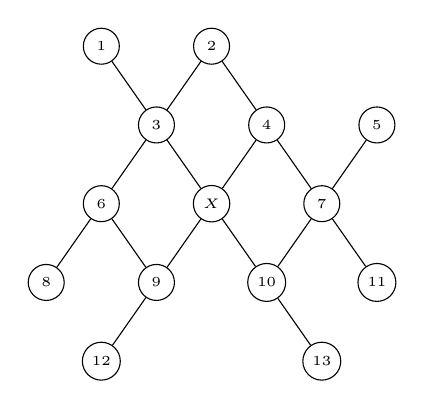
\begin{tikzpicture}
	\tiny
	\node[lightstyle,minimum size=13] (x) at (0,0) {$X$};
	\node[lightstyle,minimum size=13] (1) at (-1.4,2) {1};
	\node[lightstyle,minimum size=13] (2) at (0,2) {2};
	\node[lightstyle,minimum size=13] (3) at (-0.7,1) {3};
	\node[lightstyle,minimum size=13] (4) at (0.7,1) {4};
	\node[lightstyle,minimum size=13] (5) at (2.1,1) {5};
	\node[lightstyle,minimum size=13] (6) at (-1.4,0) {6};
	\node[lightstyle,minimum size=13] (7) at (1.4,0) {7};
	\node[lightstyle,minimum size=13] (8) at (-2.1,-1) {8};
	\node[lightstyle,minimum size=13] (9) at (-0.7,-1) {9};
	\node[lightstyle,minimum size=13] (10) at (0.7,-1) {10};
	\node[lightstyle,minimum size=13] (11) at (2.1,-1) {11};
	\node[lightstyle,minimum size=13] (12) at (-1.4,-2) {12};
	\node[lightstyle,minimum size=13] (13) at (1.4,-2) {13};
	\draw (1)--(3);
	\draw (2)--(3);
	\draw (2)--(4);
	\draw (3)--(6);
	\draw (3)--(x);
	\draw (4)--(x);
	\draw (4)--(7);
	\draw (5)--(7);
	\draw (6)--(8);
	\draw (6)--(9);
	\draw (7)--(10);
	\draw (7)--(11);
	\draw (9)--(12);
	\draw (10)--(13);
	\draw (x)--(9);
	\draw (x)--(10);
	\end{tikzpicture}
}

\newcommand{\undirectedmbsolved}
{
	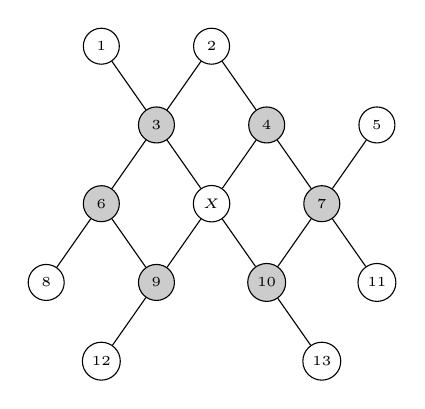
\begin{tikzpicture}
	\tiny
	\node[lightstyle,minimum size=13] (x) at (0,0) {$X$};
	\node[lightstyle,minimum size=13] (1) at (-1.4,2) {1};
	\node[lightstyle,minimum size=13] (2) at (0,2) {2};
	\node[darkstyle,minimum size=13] (3) at (-0.7,1) {3};
	\node[darkstyle,minimum size=13] (4) at (0.7,1) {4};
	\node[lightstyle,minimum size=13] (5) at (2.1,1) {5};
	\node[darkstyle,minimum size=13] (6) at (-1.4,0) {6};
	\node[darkstyle,minimum size=13] (7) at (1.4,0) {7};
	\node[lightstyle,minimum size=13] (8) at (-2.1,-1) {8};
	\node[darkstyle,minimum size=13] (9) at (-0.7,-1) {9};
	\node[darkstyle,minimum size=13] (10) at (0.7,-1) {10};
	\node[lightstyle,minimum size=13] (11) at (2.1,-1) {11};
	\node[lightstyle,minimum size=13] (12) at (-1.4,-2) {12};
	\node[lightstyle,minimum size=13] (13) at (1.4,-2) {13};
	\draw (1)--(3);
	\draw (2)--(3);
	\draw (2)--(4);
	\draw (3)--(6);
	\draw (3)--(x);
	\draw (4)--(x);
	\draw (4)--(7);
	\draw (5)--(7);
	\draw (6)--(8);
	\draw (6)--(9);
	\draw (7)--(10);
	\draw (7)--(11);
	\draw (9)--(12);
	\draw (10)--(13);
	\draw (x)--(9);
	\draw (x)--(10);
	\end{tikzpicture}
}

\newcommand{\directedmb}
{
	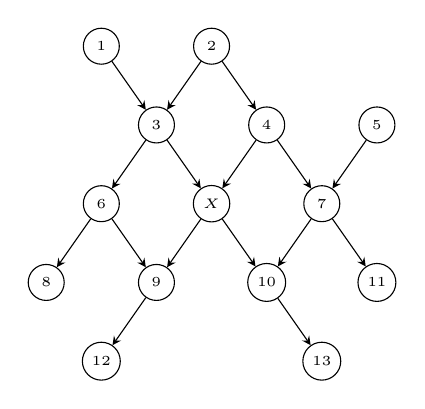
\begin{tikzpicture}
	\tiny
	\node[lightstyle,minimum size=13] (x) at (0,0) {$X$};
	\node[lightstyle,minimum size=13] (1) at (-1.4,2) {1};
	\node[lightstyle,minimum size=13] (2) at (0,2) {2};
	\node[lightstyle,minimum size=13] (3) at (-0.7,1) {3};
	\node[lightstyle,minimum size=13] (4) at (0.7,1) {4};
	\node[lightstyle,minimum size=13] (5) at (2.1,1) {5};
	\node[lightstyle,minimum size=13] (6) at (-1.4,0) {6};
	\node[lightstyle,minimum size=13] (7) at (1.4,0) {7};
	\node[lightstyle,minimum size=13] (8) at (-2.1,-1) {8};
	\node[lightstyle,minimum size=13] (9) at (-0.7,-1) {9};
	\node[lightstyle,minimum size=13] (10) at (0.7,-1) {10};
	\node[lightstyle,minimum size=13] (11) at (2.1,-1) {11};
	\node[lightstyle,minimum size=13] (12) at (-1.4,-2) {12};
	\node[lightstyle,minimum size=13] (13) at (1.4,-2) {13};
	\draw[-stealth] (1)--(3);
	\draw[-stealth] (2)--(3);
	\draw[-stealth] (2)--(4);
	\draw[-stealth] (3)--(6);
	\draw[-stealth] (3)--(x);
	\draw[-stealth] (4)--(x);
	\draw[-stealth] (4)--(7);
	\draw[-stealth] (5)--(7);
	\draw[-stealth] (6)--(8);
	\draw[-stealth] (6)--(9);
	\draw[-stealth] (7)--(10);
	\draw[-stealth] (7)--(11);
	\draw[-stealth] (9)--(12);
	\draw[-stealth] (10)--(13);
	\draw[-stealth] (x)--(9);
	\draw[-stealth] (x)--(10);
	\end{tikzpicture}
}

\newcommand{\directedmbsolved}
{
	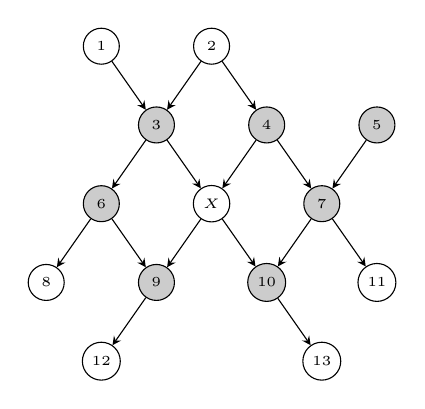
\begin{tikzpicture}
	\tiny
	\node[lightstyle,minimum size=13] (x) at (0,0) {$X$};
	\node[lightstyle,minimum size=13] (1) at (-1.4,2) {1};
	\node[lightstyle,minimum size=13] (2) at (0,2) {2};
	\node[darkstyle,minimum size=13] (3) at (-0.7,1) {3};
	\node[darkstyle,minimum size=13] (4) at (0.7,1) {4};
	\node[darkstyle,minimum size=13] (5) at (2.1,1) {5};
	\node[darkstyle,minimum size=13] (6) at (-1.4,0) {6};
	\node[darkstyle,minimum size=13] (7) at (1.4,0) {7};
	\node[lightstyle,minimum size=13] (8) at (-2.1,-1) {8};
	\node[darkstyle,minimum size=13] (9) at (-0.7,-1) {9};
	\node[darkstyle,minimum size=13] (10) at (0.7,-1) {10};
	\node[lightstyle,minimum size=13] (11) at (2.1,-1) {11};
	\node[lightstyle,minimum size=13] (12) at (-1.4,-2) {12};
	\node[lightstyle,minimum size=13] (13) at (1.4,-2) {13};
	\draw[-stealth] (1)--(3);
	\draw[-stealth] (2)--(3);
	\draw[-stealth] (2)--(4);
	\draw[-stealth] (3)--(6);
	\draw[-stealth] (3)--(x);
	\draw[-stealth] (4)--(x);
	\draw[-stealth] (4)--(7);
	\draw[-stealth] (5)--(7);
	\draw[-stealth] (6)--(8);
	\draw[-stealth] (6)--(9);
	\draw[-stealth] (7)--(10);
	\draw[-stealth] (7)--(11);
	\draw[-stealth] (9)--(12);
	\draw[-stealth] (10)--(13);
	\draw[-stealth] (x)--(9);
	\draw[-stealth] (x)--(10);
	\end{tikzpicture}
}


\begin{frame}{Markov Blanket: Undirected Graph}
\vspace{0pt}
\centering
\begin{figure}[!t]
\undirectedmb
\end{figure}
\end{frame}

\begin{frame}{Markov Blanket: Undirected Graph}
\vspace{0pt}
\centering
\begin{figure}[!t]
\undirectedmbsolved
\end{figure}
\end{frame}

\begin{frame}{Markov Blanket: Directed Graph}
\vspace{0pt}
\centering
\begin{figure}[!t]
\directedmb
\end{figure}
\end{frame}

\begin{frame}{Markov Blanket: Directed Graph}
\vspace{0pt}
\centering
\begin{figure}[!t]
\directedmbsolved
\end{figure}
\end{frame}

\begin{frame}{Equivalence of Local and Global Independencies}
\begin{itemize}
	\item We can now formulate a definition for $I_{\ell}(H)$ in terms of
	the Markov blankets of each $X \in H$:
	\[
		I_{\ell}(H) = \{(X \perp \mathcal{X} - \{X\} - \text{MB}_{H}(X)
		\;|\; \text{MB}_{H}(X)) : X \text{---} Y \notin H\}.
	\]
	\item The following three statements are equivalent for a positive
	distribution $P$:
	\begin{enumerate}
		\item $P \models I_{\ell}(H)$.
		\item $P \models I_{p}(H)$.
		\item $P \models I(H)$.
	\end{enumerate}
\end{itemize}
\end{frame}

\subsection{Distributions to Graphs}

%\begin{frame}{From Distributions to Graphs}
%\begin{itemize}
%	\item Given a distribution $P$, can we go the other way around and
%	construct a graph $H$ such that $H$ is a minimal I-map for $P$?
%	\item Doing so requires the concept of a minimal I-map, and leads to the
%	following:
%	\begin{itemize}
%		\item For positive distributions, \emph{all four conditions} ---
%		factorization and the three types of Markov assumptions --- are
%		all equivalent.
%	\end{itemize}
%	\item Refer to Chapter 4 of \cite{pgmbook} and \cite{arslides} for more
%	information.
%\end{itemize}
%\end{frame}

\begin{frame}{Distributions to Graphs}
\begin{itemize}
	\item Given a distribution $P$, can we go the other way around and
	construct a graph $H$ such that $H$ is a minimal I-map for $P$?
	\item We can satisfy $I(H)$ by visiting each node $X \in H$ and ensuring
	that the $I_{\ell}(H)$ is satisfied by observing all $Y \in
	\text{MB}_{H}(X)$.
\end{itemize}
\end{frame}

\begin{frame}{Distributions to Graphs}
\begin{itemize}
	\item By construction, $H$ satisfies $I_{\ell}(H)$ and thus is an I-map
	for $H$.
	\item Assume that $H$ is not a minimal I-map. Removing an edge in $H$
	results in some assertion $(X \perp Y \;|\; \mathcal{X} - \{X,Y\})$ not
	being reflected in $P$, violating $I_{p}(H)$.
	\item Hence, $H$ is a minimal I-map.
\end{itemize}
\end{frame}

\begin{frame}{Hammersley-Clifford Theorem}
\begin{itemize}
	\item Let $P$ be a positive distribution over $\mathcal{X}$, and $H$ a
	Markov network graph over $\mathcal{X}$. If $H$ is an I-map for $P$,
	then $P$ is a Gibbs distribution over $H$.
	\item For positive distributions, \emph{all four conditions} ---
	factorization and the three types of Markov assumptions --- are all
	equivalent.
\end{itemize}
\end{frame}

%\newcommand{\trigraph}
%{
%	\subfloat[][(a)]
%	{%
%		\begin{tikzpicture}
%		\scriptsize
%		\node[darkstyle,minimum size=20] (b) at (0,1.5) {$B$};
%		\node[darkstyle,minimum size=20] (a) at (-1,0) {$A$};
%		\node[darkstyle,minimum size=20] (c) at (1,0) {$C$};
%		\draw (a)--(b);
%		\draw (b)--(c);
%		\draw (c)--(a);
%		\end{tikzpicture}
%	}%
%	\hspace{0.5cm}
%	\subfloat[][(b)]
%	{%
%		\begin{tikzpicture}
%		\scriptsize
%		\node[darkstyle,minimum size=20] (b) at (0,1.5) {$B$};
%		\node[darkstyle,minimum size=20] (a) at (-1,0) {$A$};
%		\node[darkstyle,minimum size=20] (c) at (1,0) {$C$};
%		\node[factorstyle,minimum size=20] (v1) at (-1.6,1.5)
%			{$V_{\phi_{1}}$};
%		\node[factorstyle,minimum size=20] (v2) at (1.6,1.5)
%			{$V_{\phi_{2}}$};
%		\node[factorstyle,minimum size=20] (v3) at (0,-1.2)
%			{$V_{\phi_{2}}$};
%		\draw (v1.south)--(a);
%		\draw (a)--(v3.west);
%		\draw (v2.south)--(c);
%		\draw (c)--(v3.east);
%		\draw (v1.east)--(b);
%		\draw (b)--(v2.west);
%		\end{tikzpicture}
%	}%
%	\hspace{0.5cm}
%	\subfloat[][(c)]
%	{%
%		\begin{tikzpicture}
%		\scriptsize
%		\node[darkstyle,minimum size=20] (b) at (0,1.5) {$B$};
%		\node[darkstyle,minimum size=20] (a) at (-1,0) {$A$};
%		\node[darkstyle,minimum size=20] (c) at (1,0) {$C$};
%		\node[factorstyle,minimum size=20] (v) at (0,-1.2) {$V_{\phi}$};
%		\draw (a)--(v.west);
%		\draw (c)--(v.east);
%		\draw (b)--(v.north);
%		\end{tikzpicture}
%	}
%}
%
%\begin{frame}{Factor Graphs}
%\setlength{\topsep}{0pt}
%\setlength{\partopsep}{0pt}
%\vspace{0pt}
%\centering
%\begin{figure}[!t]
%\resizebox{0.8\textwidth}{!}{\trigraph}
%\end{figure}
%\begin{itemize}
%	\item Given graph (a), we cannot fully determine the Gibbs
%	parameterization.
%	\item Factors in the network could be over one variable, two variables,
%	or all three variables, as there are three kinds of cliques in the
%	graph.
%\end{itemize}
%\end{frame}
%
%\begin{frame}{Factor Graphs}
%\setlength{\topsep}{0pt}
%\setlength{\partopsep}{0pt}
%\vspace{0pt}
%\centering
%\begin{figure}[!t]
%\resizebox{0.8\textwidth}{!}{\trigraph}
%\end{figure}
%\begin{itemize}
%	\item Factor graphs only contain edges between variable nodes (circles)
%	and factor nodes (boxes).
%	\item This makes the structure of the Gibbs parameterization explicit,
%	and ensures that each node $V_{\phi}$ is associated with exactly one
%	factor $\phi$ involving its neighbors.
%\end{itemize}
%\end{frame}

\subsection{Log-Linear Models}

\begin{frame}{Log-Linear Models}
\begin{itemize}
	\item Instead of encoding factors as complete tables over their scope,
	we can use an alternate parameterization that can make context-specific
	structure more apparent.
	\item We can rewrite a factor $\phi(\boldsymbol{D})$ as
	\[
		\phi(\boldsymbol{D}) = \text{exp}(-\epsilon(\boldsymbol{D})),
	\]
	where $\phi(\boldsymbol{D}) = -\text{ln}\phi(\boldsymbol{D})$.
	\item The logarithmic representation ensures that the distribution is
	positive.
\end{itemize}
\end{frame}

\begin{frame}{Log-Linear Models}
\begin{itemize}
	\item A distribution $P$ is a log-linear model over a Markov network $H$
	if it is associated with
	\begin{itemize}
		\item a set of features $F = \{f_{1}(\boldsymbol{D}_{1}),
		\ldots, f_{k}(\boldsymbol{D}_{k})\}$, where each
		$\boldsymbol{D}_{i}$ is a complete subgraph in $H$, and
		\item a set of weights $w_{1}, \ldots, w_{k}$,
	\end{itemize}
	such that
	\[
		P(X_{1}, \ldots, X_{n}) =
		\frac{1}{Z}\text{exp}\left[-\sum_{i=1}^{k}
		w_{i}f_{i}(\boldsymbol{D}_{i})\right].
	\]
\end{itemize}
\end{frame}

\begin{frame}{Log-Linear Models: The Ising Model}
\begin{itemize}
	\item The Ising model is a model for the energy of a particular system
	involving a system of interacting atoms.
	\item Each atom is associated with a binary variable $X_{i} = \{+1,
	-1\}$, whose value defines the direction of the atom's spin.
	\item The energy function associated with the edges is defined by
	\[
		\epsilon_{ij}(x_{i}, x_{j}) = w_{i,j}x_{i}x_{j}.
	\]
	\item When two atoms $X_{i},X_{j}$ have the same spin, they make a
	contribution $w_{i,j}$; otherwise, they make a contribution $-w_{i,j}$.
	\item We also include single node potentials $u_{i}$ that bias a
	particular atom to have one spin or another.
\end{itemize}
\end{frame}

\begin{frame}{Log-Linear Models: The Ising Model}
\begin{itemize}
	\item The energy distribution is given by the definition of the
	log-linear model:
	\[
		P(\xi) = \frac{1}{Z}\left(-\sum_{i<j}w_{i,j}x_{i}x_{j} -
		\sum_{i}u_{i}x_{i}\right).
	\]
	\item When $w_{i,j} > 0$ the model prefers to align the spin of the two
	atoms, and the interaction is called \emph{ferromagnetic}.
	\item When $w_{i,j} < 0$, the interaction is called
	\emph{antiferromagnetic}.
	\item When $w_{i,j} = 0$, the atoms are non-interacting.
	\item Also related is the Boltzmann machine, which has gained wide
	popularity in deep learning.
\end{itemize}
\end{frame}

\newcommand{\isingmodel}
{
	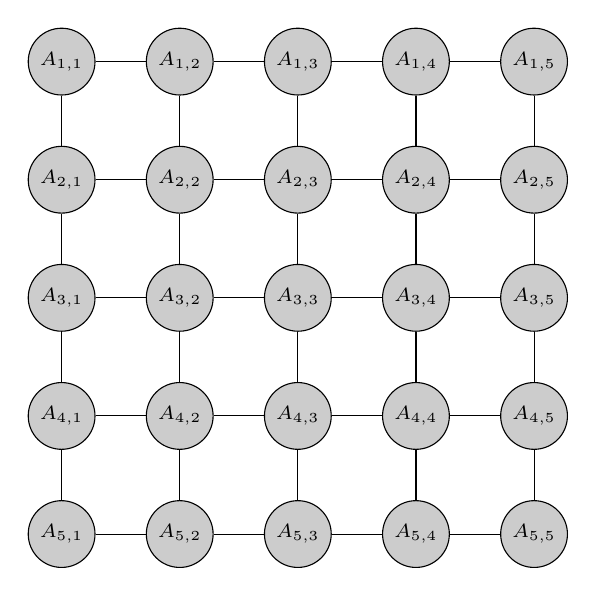
\begin{tikzpicture}
	\scriptsize
	\foreach \x in {0,...,4}
	\foreach \y in {0,...,4}
	{
		\pgfmathtruncatemacro{\r}{5-\y}
		\pgfmathtruncatemacro{\c}{\x+1}
		\node[darkstyle] (\x\y) at (1.5*\x,1.5*\y) {$A_{\r,\c}$};
	}
	\foreach \x in {0,...,4}
	\foreach \y [count=\yi] in {0,...,3}
	\draw (\x\y)--(\x\yi) (\y\x)--(\yi\x);
	\end{tikzpicture}
}

\begin{frame}{Log-Linear Models: The Ising Model}
\begin{center}
\isingmodel
\end{center}
\end{frame}

\begin{thebibliography}{11}
\bibitem{pgmbook}
Daphne Koller and Nir Friedman,
\emph{Probabilistic Graphical Models: Principles and Techniques},
MIT Press,
1st Edition,
2009.
\bibitem{pgmslides}
David Sontag, lecture slides on Probabilistic Graphical Models.
Accessible at \url{http://cs.nyu.edu/~dsontag/courses/pgm12/}.
\bibitem{nirslides}
Nir Friedman, lecture slides on the theory of Bayesian networks.
Accessible at \url{classes.soe.ucsc.edu/cmps290c/Spring04/paps/nir2.pdf}.
\end{thebibliography}

\end{document}
